\subsection{\(\mathcal{GP}\) Models for Catalytic Responses}
A \(\mathcal{GP}\) is a distribution over smooth latent functions \(g: \mathcal{X} \rightarrow \mathbb{R}\). 
Assuming the observation model \(p(y\vert g)\) is known, the standard approach is to use non-parametric Bayesian approach by placing a \(\mathcal{GP}\) distribution over \(g\), i.e. \(p(g)=\mathcal{GP}\big(\mu(x),k(x,x')\big)\). 
Here \(\mu(x):\mathcal{X}\rightarrow \mathbb{R}\) is a mean function and \(k(x,x'):\mathcal{X}\times\mathcal{X}\rightarrow \mathbb{R}\) is a covariance function. 
A function-space viewpoint provides an intuitive explanation of \(\mathcal{GP}\) as vector space of functions in a chosen (potentially non-linear) feature space which \(\phi(x)\) as a basis. 
In the function space representation, the observation model plays the role of weights \(W\) with function \(g\) represented using \(g(x) = \phi(x)^{\top}W\). 
It can be shown~(see Supplementary Information) that \(\phi(x)\) can be implicitly defined using the covariance function \(k(x,x')\) between pair of inputs \(x,x'\in\mathcal{X}\) and a mean function \(\mu(x)\) of \(W\)~\footnote{for this reason we use \(k(x,x')\) and basis function of \(\mathcal{GP}\) interchangeably in this paper}. 
The mean function \(\mu\) encodes an average behavior of the function \(g\). 
The covariance function \(k(x,x')\) encodes the correlations between outputs \(g(x), g(x')\) for any given pair of input points~(\(x,x'\)). 
In this chapter, the concatenated vector of the parameters \(\mu(x)\) and \(k(x,x')\) is denoted as \(\theta\).
Once we select a \(\mathcal{GP}\) encoding our prior beliefs, we use Bayes rule to update our posterior \(p(g\vert \mathcal{D})\) conditioned on observed data \(\mathcal{D}=(\textbf{X},\textbf{y})\) where \(\textbf{y}\) are the discrete evaluations of function \(g\) at inputs \(\textbf{X}\). 
For more information on \(\mathcal{GP}\), readers are referred to~\cite{williams2006gaussian}.

A typical response from a cyclic voltammetry experiment is represented as a function \(I(t,v)\) with \(I\) being the current response collected at a time (\(t\)) for a time dependent applied voltage \(v=V(t)\). 
The voltage load \(V(t)\) is typically chosen to be linear and the voltammetry is often referred as direct current voltammetry~\cite{li2019application}.
Classification of a CV into an S-shape (or not S-shape) can be looked at as determining a model evidence of a function defined by CV curve \( (v,t) \mapsto I\) under a \(\mathcal{GP}\) function space with observed data \(\mathcal{D}\) given by the discrete CV curve \(\textbf{X} = I, \textbf{y}=(v,t)\). 
The covariance of a CV curve gives rise to the basis functions in the \(\mathcal{GP}\) space and the time-voltage grid becomes the input space where the function is evaluated.
For any given CV curve, its representation in the \(\mathcal{GP}\) function space  is obtained by finding a \(\theta\) that maximize the posterior probability \(p(\textbf{X} = I|\textbf{y}=(v,t))\)~\footnote{we use the \textit{maximum a posteriori} or MAP estimation}.
The \(\mathcal{GP}\) model is chosen with a \textit{non-stationary} covariance as a target model~\(\mathcal{M}_2\). 
It follows from the reproducing kernel Hilbert space~(RKHS) theorem~(Ch 12.4 in \cite{mathML}) that any smooth function can be represented using a kernel or a covariance function.
Thus for the null model~(\(\mathcal{M}_1\)), it is sufficient to use a \(\mathcal{GP}\) with smoothness controllable covariance function. 
A brief overview of the covariance functions selected as basis functions is described below.
For both models \(\mathcal{M}_1\) and \(\mathcal{M}_2\), the mean function is chosen to be \(\mu(x)=0 \) as we normalize the response curves \(I(v,t)\) to be with in \((0,1)\) and expect the covariance function to determine the shape of the CV curve. 

\subsubsection{Squared Exponential Covariance}
The commonly known \textit{squared exponential kernel}~(in~\Cref{eq:covSEard} and~\Cref{fig:covSEard}) is used as a covariance model for \(\mathcal{M}_1\) where the resulting feature map \(\phi(x)\) forms a basis for functions that are smooth and stationary.
\begin{equation}
    k(x,x')=\sigma_f^2 \exp((x-x')^{\top}\Lambda^{-1}(x-x'))
    \label{eq:covSEard}
\end{equation}
In~\Cref{eq:covSEard}, \(\sigma_f\) is scaling parameter, and \(\Lambda\) is a diagonal matrix with each entry as a length scale for the corresponding dimension of \(x,x'\in \mathcal{X}\). 
The left panel of \Cref{fig:covSEard} depicts five samples drawn at random from the \(\mathcal{GP}\) with the covariance in~\Cref{eq:covSEard}.% The input to the function \(g\) s \(x\) and real valued outputs as \(g(x)\). 
The right panel of the same figure depicts the covariance function visualized on a uniform grid of \(\mathcal{X}\times\mathcal{X}\) as contours. 
From~\Cref{fig:covSEard}, it can be seen that the covariance is stronger~(\(\approx 1\)) between inputs with Euclidean norm~(i.e. distance) less than a length scale controlled by the parameter \(\Lambda\).

\begin{figure}[h]
    \centering
    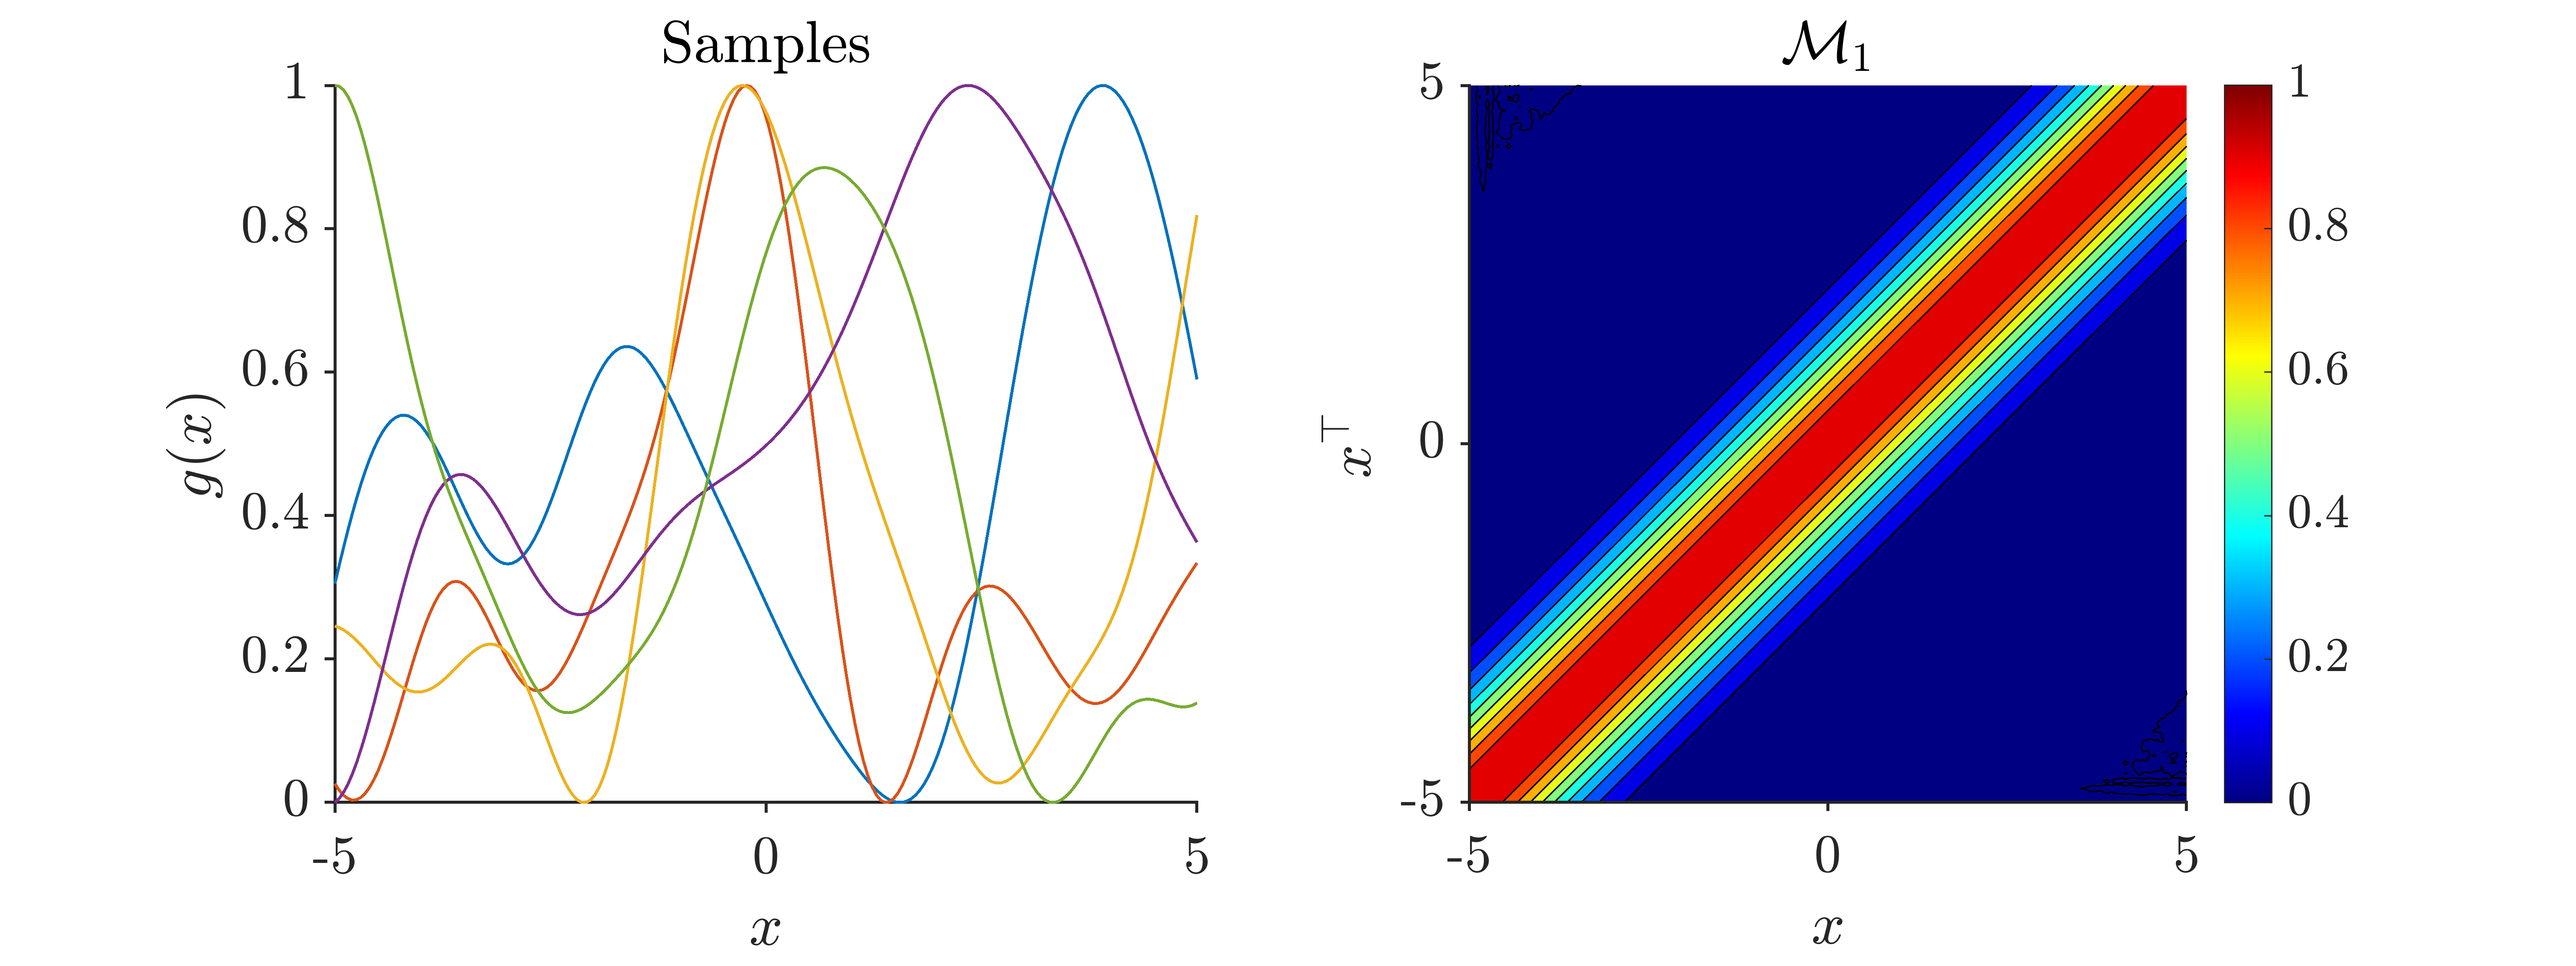
\includegraphics[scale=0.5]{Chapter-3/figures/Model1.png}
    \caption{A pictorial representation of~\Cref{eq:covSEard}. Left panel: five samples drawn at random from the \(\mathcal{GP}\) built using~\Cref{eq:covSEard}, captures the smooth and locally correlated nature of the \(\mathcal{GP}\). Right panel: a contour plot depicting correlations between outputs of one-dimensional vectors \(x,x' \in \mathcal{X}\). Color code represents the covariance \(k(x,x')\) with red representing high covariance i.e. output values \(g(x), g(x')\) are highly correlated and vice-versa. }
    \label{fig:covSEard}
\end{figure}

\subsubsection{Neural Network Covariance}
The target model uses neural network covariance kernel to build a \(\mathcal{GP}\) function space representation referred as model~\(\mathcal{M}_2\)(shown in~\Cref{eq:covNNone} and~\Cref{fig:covNNone}).
The S-shape responses have a non-stationary covariance and hence a covariance that is effective in handling rapidly changing signals would be a good choice. 

\begin{align}
        k(x,x') &= \sigma_f^2 \sin^{-1}\left({\frac{x^{\top}\Lambda^{-2}x'}{\sqrt{h(x)h(x')}}}\right) \label{eq:covNNone}\\
        h(x) &= 1+x^{\top}\Lambda^{-2}x \nonumber
\end{align}
In~\Cref{eq:covNNone}, \(\sigma_f\) is scaling parameter, and \(\Lambda\) is a diagonal matrix with each entry as a length scale.
\Cref{fig:covNNone} is analogues to~\Cref{fig:covSEard} and it can be seen that the covariance is high~(\(\approx 1\)) in two blocks of input locations that are separated by a completely uncorrelated input locations~(covariance \(\approx 0\)). 
This is in contrast to \(\mathcal{M}_1\) where the covariance is determined by some form of distance between input points. 
\begin{figure}[h]
    \centering
    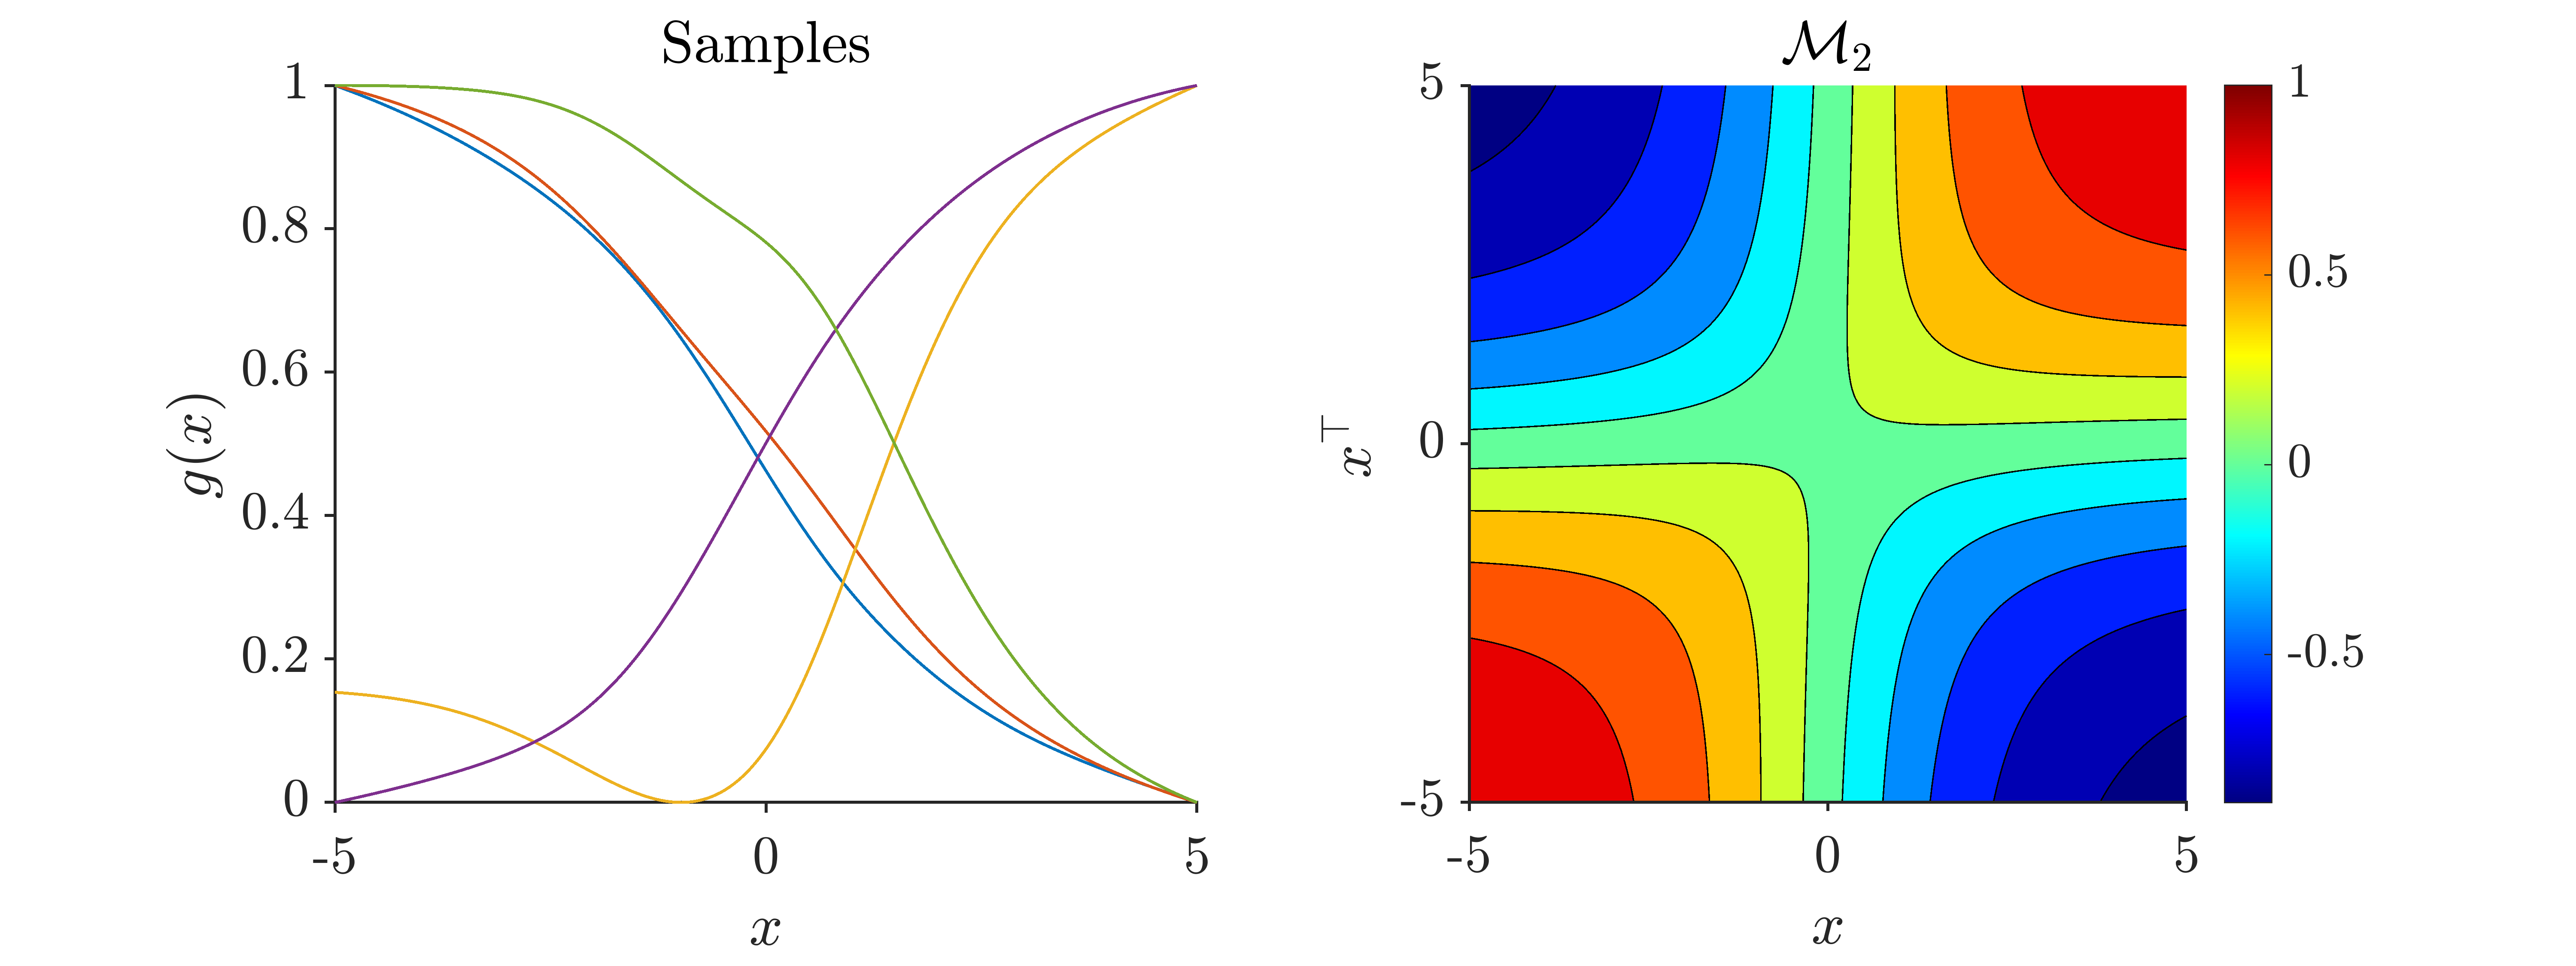
\includegraphics[scale=0.5]{Chapter-3/figures/Model2.png}
    \caption{A pictorial representation of~\Cref{eq:covNNone}. Left panel: five samples drawn at random from the \(\mathcal{GP}\) built using~\Cref{eq:covNNone}, captures the non-stationary nature nature of the \(\mathcal{GP}\) signified by constant values and sharp rises in the response values. Right panel: a contour plot of covariance between two one-dimensional vectors \(x,x' \in \textbf{X}\) as inputs. A positive value for \(k(x,x')\) signifies that output values \(g(x), g(x')\) are highly correlated and vice-versa. }
    \label{fig:covNNone}
\end{figure}

